% ============================================================================
\section{Detector, Data and Inputs}
\label{app:data}
% ============================================================================

\subsection{Trigger rate and latency context}
\label{app:trigger_context}
Proton bunches cross at \SI{40}{MHz}, while front-end buffers retain detector information for only a few microseconds. Readout and storage bandwidth cannot accommodate every collision, so the Level-1 trigger makes a fixed-latency hardware decision and reduces the accepted rate to about \SI{100}{kHz}~\cite{atlas_trigger_run3}. It uses fast, reduced detector information rather than the full offline readout; the eFEX groups calorimeter deposits into candidate TOBs~\cite{atlas_phase1_tdr}. The accepted rate is shared among physics selections. Since ordinary background dominates, each selection's rate allocation motivates a background-acceptance constraint. The $0.5\%$ event-level budget used here is the specification of this study, not a universal conversion from an LHC rate to a sample acceptance. Comparisons must use a common background sample and operating point.

\subsection{Tau decays and the QCD background}
\label{app:tau_context}
The tau is a short-lived lepton of mass $m_\tau\simeq\SI{1.777}{GeV}$~\cite{pdg2024}; its decay products, rather than the tau itself, reach the detector. Tau pairs arise in processes including $Z$ and Higgs decays. About $65\%$ of tau decays are hadronic, producing a neutrino and a small number of hadrons, commonly one or three charged prongs together with neutral pions that decay into photon pairs. Electron and muon decays are handled by other triggers; throughout this paper, ``tau'' denotes the hadronic channel. The neutrino is invisible, while the visible hadrons and photons produce a narrow shower. QCD jets are vastly more frequent, typically wider and richer in hadronic activity, yet overlap strongly with tau showers at low energy. This combination of class imbalance and ambiguous soft showers motivates shape information in addition to energy.

\subsection{Sample provenance and candidate construction}
\label{app:sample_provenance}
The samples are Monte Carlo simulations from the resimulated FEX truth/all-cell production, providing detector-level calorimeter information and generator-level truth. The exact production identifiers are:
\begin{itemize}
  \item \textbf{Signal ($\tau$ events):}\newline
  {\footnotesize\nolinkurl{user.dreikher.801002.Py8EG_A14NNPDF23LO_Gammatautau_MassWeight.e8557_s4422_r16130}}
  \item \textbf{Background (QCD dijet events):}\newline
  {\footnotesize\nolinkurl{user.dreikher.801165.Py8EG_A14NNPDF23LO_jj_JZ0.e8557_s4422_r16130}}
\end{itemize}
% Provenance: current production details supplied by the physics collaborators.
% Older supporting notes describe earlier samples/representations; do not infer
% additional generator settings, pile-up conditions or cuts for this production.
The simulated eFEX, part of the Level-1 calorimeter trigger, supplies tau TOBs as candidate seeds. Within each event, TOBs are sorted by $\ptTOB$ and at most six are retained; events with no TOBs are discarded. Their $\ptTOB$, $\eta$ and $\phi$ are retained as candidate-level quantities.

For each retained TOB in the signal sample, the closest visible truth $\tau$ is found using $\Delta R=\sqrt{(\Delta\eta)^2+(\Delta\phi)^2}$, with periodic wrapping of $\Delta\phi$. The object label is positive only for $\Delta R<0.15$. Unmatched signal-sample TOBs and all QCD-sample TOBs are negative. Thus, sample membership alone does not determine the object label. Truth information is used for labels, loss weights and offline evaluation, never as an inference input.

\paragraph{Calorimeter binning.}
Cells are selected within $|\Delta\eta|<0.15$ and $|\Delta\phi|<0.15$ of the TOB centre. Their transverse energies are separated into four electromagnetic layers (EM0--EM3) and one combined hadronic layer, each binned into $3\times3$ cells to form the $5\times3\times3$ tensor. A separate $12\times12$ grid represents EM2 over the \emph{same} angular region. Transverse energies of cells assigned to the same bin are summed. The EM2 image therefore increases spatial resolution, not angular coverage; a $3\times3$ window within that image is not the full coarse $3\times3$ EM2 layer.

\subsection{Calorimeter layers}
\Cref{tab:layers} summarises the role of each layer in the core tensor. The layer order in the tensor, EM0 to HAD, follows the depth of the calorimeter. Physically, a hadronic $\tau$ decay deposits the photons of its $\pi^0$ mesons mainly in EM1--EM2, and part of the energy of its charged pions in EM2--EM3 and HAD. Its narrow opening angle keeps most of the energy in the central tower. A QCD jet carries more hadrons and more particles, so it is wider in $(\eta,\phi)$ and deeper in the calorimeter.

\begin{table}[h]
  \centering
  \caption{Longitudinal layers of the per-object calorimeter window.}
  \label{tab:layers}
  \small
  \begin{tabularx}{\linewidth}{@{}llXl@{}}
    \toprule
    Layer & Detector part & Physical role & Representation \\
    \midrule
    EM0 & presampler & energy lost in material upstream & $3\times3$ towers \\
    EM1 & EM front (strips) & fine $\eta$ segmentation; resolves $\pi^0\to\gamma\gamma$ & $3\times3$ towers \\
    EM2 & EM middle & bulk and core of EM showers & $3\times3$ towers, $12\times12$ cells \\
    EM3 & EM back & tail of energetic EM showers & $3\times3$ towers \\
    HAD & hadronic calorimeter & energy of charged hadrons & $3\times3$ towers \\
    \bottomrule
  \end{tabularx}
\end{table}

\subsection{Coordinates and kinematic variables}
\label{app:coordinates}
The beam defines the $z$ axis, and the plane perpendicular to it is the \emph{transverse} plane.
\begin{itemize}
  \item \textbf{Azimuth} $\phi\in[-\pi,\pi)$ is the angle around the beam in the transverse plane.
  \item \textbf{Pseudorapidity} $\eta=-\ln\tan(\theta/2)$ is a monotone function of the polar angle $\theta$ measured from the beam axis. $\eta=0$ is perpendicular to the beam, and $|\eta|$ grows towards the beam. All TOBs in our data have $|\eta|<2.5$. Equal steps in $\eta$ correspond to roughly equal particle densities, which is why calorimeter towers have a fixed size of $0.1\times0.1$ in $(\eta,\phi)$.
  \item \textbf{Transverse momentum} $\pT=|\vec p|\sin\theta$ is the momentum component perpendicular to the beam. Before the collision the transverse momentum is zero, so $\pT$ is the natural scale for the hard products of a collision. The eFEX estimates $\ptTOB$ from the calorimeter energy of the object (in GeV, in steps of \SI{100}{MeV}, with a minimum of \SI{5}{GeV}). The true $\pT$ of a $\tau$ comes from the simulation and is not available in real data.
  \item \textbf{Angular distance} between two objects is $\Delta R=\sqrt{\Delta\eta^2+\Delta\phi^2}$, with $\Delta\phi$ wrapped to $[-\pi,\pi)$.
\end{itemize}
In the \CP\ inputs, $\eta$ and $\phi$ are taken relative to the highest-$\ptTOB$ object of the event, so they describe where an object lies with respect to the leading activity. TOB positions are given at tower resolution. The BDT score is a per-TOB boosted-decision-tree output supplied with the eFEX objects.

\subsection{Per-object columns}
\Cref{tab:inputs} lists every column available per object and how it may be used. Energies are stored in MeV and converted to GeV for evaluation. The $12\times12$ EM2 image sums exactly to the EM2 $3\times3$ core, so the two are views of the same energy at different granularity. For truth-matched $\tau$ objects the median of $\ptTOB/\pttruth$ is $0.59$, which reflects the energy carried away by the neutrino and the TOB energy scale.

\begin{table}[h]
  \centering
  \caption{Columns per object and how they may be used. ``Input'' columns may feed a network. ``Truth'' columns are used only for labels, loss weights and offline evaluation.}
  \label{tab:inputs}
  \small
  \begin{tabularx}{\linewidth}{@{}lXl@{}}
    \toprule
    Column & Content & Use \\
    \midrule
    \code{X\_tensors} & core tensor, $5\times3\times3$ cell energies (EM0--EM3, HAD) & input \\
    \code{X\_em2\_tensors} & EM2 image, $12\times12$ cell energies & input \\
    \code{tob\_pt} & eFEX TOB transverse momentum ($\SI{100}{MeV}$ steps, $\geq\SI{5}{GeV}$) & input / baseline \\
    \code{tob\_eta}, \code{tob\_phi} & TOB position (tower resolution); used relative to the leading TOB & input \\
    \code{tob\_bdt} & eFEX BDT score & input \\
    \code{eventNumber}, \code{tob\_index} & event identifier and TOB slot ($0$--$5$) & grouping only \\
    \code{Type} & sample of origin (signal or background) & grouping only \\
    \code{signal} & truth match to a hadronic $\tau$ & truth (label) \\
    \code{truth\_pt} & true $\tau$ transverse momentum & truth (weights, eval.) \\
    \code{prongs} & number of charged decay products & truth (analysis) \\
    \bottomrule
  \end{tabularx}
\end{table}

\subsection{Event-level splits}
The counts below refer to the retained analysis dataset rather than the total generated production. Events are identified by (sample, event number), since identifiers can repeat between the signal and background samples.
Each of the three seeds shuffles the complete events and splits them $70/10/20\%$ into training, validation and test sets. \Cref{tab:seed_splits} shows that every split reproduces the composition of the full dataset: the fraction of signal events stays within $0.6$ percentage points and the median true $\tau$ $\pT$ within $\SI{0.5}{GeV}$ of the full-sample values.

\begin{table}[h]
  \centering
  \caption{Composition of every event split. Signal-event fraction, truth-$\tau$ fraction among all objects, and median true $\pT$ of truth $\tau$ objects.}
  \label{tab:seed_splits}
  \small
  \begin{tabular}{@{}lccc@{\qquad}ccc@{\qquad}ccc@{}}
    \toprule
    & \multicolumn{3}{c}{Signal events [\%]} & \multicolumn{3}{c}{$\tau$ / objects [\%]} & \multicolumn{3}{c}{Median $\tau$ $\pT$ [GeV]} \\
    Seed & train & val & test & train & val & test & train & val & test \\
    \midrule
    42  & 22.48 & 22.73 & 22.57 & 6.12 & 6.19 & 6.15 & 42.0 & 42.2 & 41.4 \\
    123 & 22.50 & 23.06 & 22.35 & 6.13 & 6.26 & 6.09 & 41.9 & 42.0 & 42.0 \\
    456 & 22.52 & 22.41 & 22.60 & 6.13 & 6.11 & 6.15 & 41.9 & 42.1 & 41.7 \\
    \midrule
    Full dataset & \multicolumn{3}{c}{22.53} & \multicolumn{3}{c}{6.13} & \multicolumn{3}{c}{41.9} \\
    \bottomrule
  \end{tabular}
\end{table}

\subsection{Dataset statistics}
\begin{table}[h]
  \centering
  \caption{Event-level split for seed~42. Complete events are assigned to one split. The last column is the largest number of background events that may fire under the $0.5\%$ event-level budget.}
  \label{tab:data_stats}
  \small
  \begin{tabular}{@{}lrrrrr@{}}
    \toprule
    Split & Signal events & Background events & Objects & Truth $\tau$ objects & Max.\ firing bkg.\ events \\
    \midrule
    Train      & 50{,}588 & 174{,}410 & 1{,}265{,}650 & 77{,}498 & 872 \\
    Validation &  7{,}307 &  24{,}835 &   180{,}757   & 11{,}184 & 124 \\
    Test       & 14{,}509 &  49{,}777 &   361{,}685   & 22{,}239 & 248 \\
    \midrule
    Total      & 72{,}404 & 249{,}022 & 1{,}808{,}092 & 110{,}921 & -- \\
    \bottomrule
  \end{tabular}
\end{table}

The median true $\pT$ of truth $\tau$ objects is $\SI{41.9}{GeV}$. The quartiles are $25.6$ and $\SI{84.1}{GeV}$. Above $\SI{25}{GeV}$ the spectrum falls approximately as $t^{-2}$: in the training split the $25$--$30\GeV$ bin contains $8.3$ times more $\tau$ objects than the $95$--$100\GeV$ bin. The test set contains $5{,}145$, $5{,}341$, $3{,}705$, $3{,}199$ and $794$ truth $\tau$ objects in the bands $10$--$25$, $25$--$40$, $40$--$60$, $60$--$100$ and $100$--$120\GeV$. The validation set contains $2{,}458$, $2{,}714$, $1{,}937$, $1{,}548$ and $391$. Above $\SI{60}{GeV}$ a $5\GeV$ validation window holds only $90$--$250$ truth $\tau$ objects, so a single object moves its efficiency by $0.4$--$1.1$ percentage points. This resolution limit shaped several design choices (\cref{app:or,app:constrained}).

\subsection{Energy-conditioned compactness}
\begin{figure}[h]
  \centering
  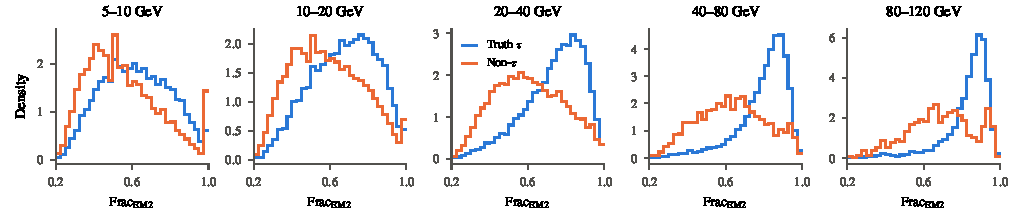
\includegraphics[width=\linewidth]{figures/fig_frac_conditioned.pdf}
  \caption{$\Frac$ for truth $\tau$ and non-$\tau$ objects in fixed $\ptTOB$ intervals (training split, normalised per class). The separation remains inside every interval and grows with energy, so the feature carries shape information beyond the energy scale.}
  \label{fig:frac_conditioned}
\end{figure}
